\shorthandoff{"}
\chapter{Methodik}
\label{ch:methodik}

\section{Forschungsart}
\label{ch:methodik:art}
Um die Forschungsfrage der vorliegenden Master-Thesis zu untersuchen, wird eine quantitative Forschungsarbeit in Form eines Experiments durchgeführt. In diesem Kontext wird ein Empfehlungssystem entwickelt, welches sowohl uni- als auch bilaterale Vorschläge zur Besetzung offener Projektpositionen erzeugt. Für beide Ansätze werden dieselben Projektbeschreibungen und Mitarbeiter als Eingabe verwendet. Die beiden Empfehlungsverfahren unterscheiden sich lediglich in der Art, in welcher sie die vorhandenen Angestellten für die eingegebenen Stellen sortieren.

Zur Beantwortung der Forschungsfrage wird eine Fallstudie mit Projektmanagern und -mitarbeitern durchgeführt. Die Mitarbeiter des Unternehmens erhalten Übersichten über vorausgewählte Projektpositionen. Daraufhin bewerten sie auf einer vordefinierten Skala, wie zufrieden sie mit einer Tätigkeit auf den vorliegenden Projektpositionen wären. Dabei wird überprüft, ob das bilaterale Empfehlungssystem die Angestellten für die Stellen höher positioniert, bei welchen diese eine hohe Zufriedenheit erwarten bzw. niedriger positioniert, wenn diese eine geringe Zufriedenheit prognostizieren.

Die Projektmanager erhalten die sortierten Mitarbeiter beider Empfehlungsansätze für die vorausgewählten Projektpositionen in Form von Listen. Hierbei ist nicht vermerkt, welche Vorschläge über den uni- bzw. den bilateralen Ansatz erzeugt wurden. Die Projektmanager bewerten auf einer vordefinierten Skala, welche Arbeitsleistung sie von denen in der vorliegenden Reihenfolge dargestellten Mitarbeitern für die jeweiligen Stellen erwarten. Dabei wird evaluiert, wie sie die erwartete Leistung der vorgeschlagenen Angestellten des bilateralen Ansatzes im Vergleich zur unilateralen Variante bewerten.

Im Rahmen der vorliegenden Master-Thesis wird ausschließlich der komplementäre \ac{PEFit} auf Facetten-Ebene betrachtet. Hierbei werden einzig die für offene Projektpositionen benötigten Kompetenzen zur Bestimmung der Kongruenz herangezogen. Weitere Faktoren wie Kundennamen oder Branchen werden nicht berücksichtigt. Im Sinne des ergänzenden \acp{PEFit} wird vorausgesetzt, dass eine grundlegende Übereinstimmung der Werte von Mitarbeitern und Unternehmen bzw. Projekttätigkeiten bereits vor Anstellung der Arbeitnehmer überprüft wurde.

Durchgeführt werden das Experiment und die Fallstudie mit Projektmanagern und Mitarbeitern des Fachbereichs \JES der EXXETA AG mit Hauptsitz in Karlsruhe. Das Unternehmen ist spezialisiert auf IT-Beratungsleistungen und arbeitet vorrangig projektbasiert. Dementsprechend ist das Zuordnen passender Angestellter zu offenen Projektpositionen in diesem Betrieb eine häufig auftretende Aufgabe.

\section{Verwendete Daten des Unternehmens}
\label{ch:methodik:versuchsaufbau}
Die Mitarbeiter der EXXETA AG pflegen ihre Kompetenzen im Intranet des Unternehmens. Dort steht eine Liste mit \anzFaehigkeiten Fähigkeiten, wie beispielsweise "Java", "DSGVO" und "Digitale Transformation", zur Verfügung. Diese können die Angestellten über die in Abbildung \ref{fig:methodik:versuchsaufbau:daten:abb1} dargestellte Skala bewerten.

\begin{figure}[h]
	\centering
	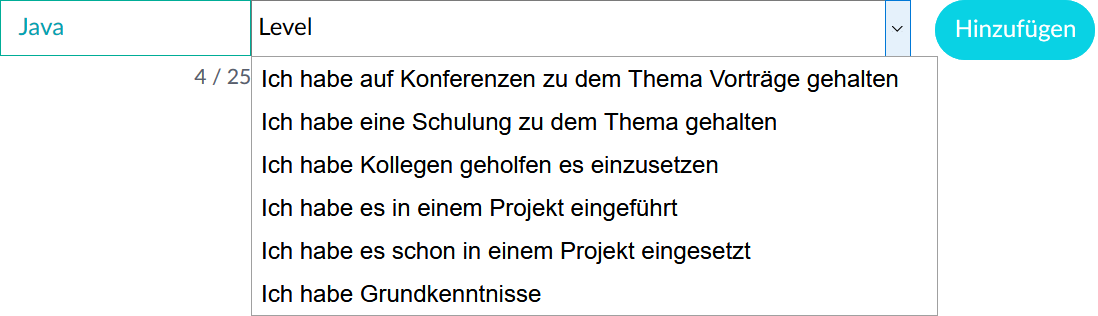
\includegraphics[width=1\textwidth]{gfx/skill-level.png}
	\caption{Hinzufügen einer Fähigkeit mit Angabe des entsprechenden Kenntnisniveaus im EXXETA-Intranet}
	\label{fig:methodik:versuchsaufbau:daten:abb1}
\end{figure}

%Die Abstufungen in Abbildung \ref{fig:methodik:versuchsaufbau:daten:abb1} werden beim Speichern in ganzzahlige Werte von \nullWert ("Ich habe Grundkenntnisse") bis fünf ("Ich habe auf Konferenzen zu dem Thema Vorträge gehalten") übertragen.
Aufgrund der klaren Beschreibungen der einzelnen Stufen in Abbildung \ref{fig:methodik:versuchsaufbau:daten:abb1} kann der in Kapitel \ref{ch:empfehlungssysteme:cf:speicherbasiert} angesprochene Bias bei der Selbsteinschätzung weitgehend ausgeschlossen werden. Außerdem ist es in der vorliegenden Problemstellung gut möglich, dass einzelne Mitarbeiter ihre Kompetenzen bewusst besser oder schlechter bewerten als andere Kollegen. Dieser Sachverhalt ist insbesondere auf längere Berufserfahrung zurückzuführen. Aus diesen Gründen wird bei der Empfehlungsbestimmung auf eine Mittelwert-Zentrierung verzichtet.

Damit Projektmanager Vorschläge erhalten können, müssen sie die für offene Projektpositionen nachgefragten Fähigkeiten mitsamt der benötigten Kenntnisniveaus festlegen. Die relevanten Kompetenzen bestimmen die Verantwortlichen in der Regel anhand eingehender Projektanfragen, welche Kunden in unstrukturierter Form, beispielsweise per Telefon oder E-Mail, einreichen. Derartige Anfragen werden täglich in großer Anzahl bearbeitet. Daher wird es für den praktischen Einsatz als sehr umständlich bewertet, wenn Verantwortliche für jede Projektanfrage sämtliche Fähigkeiten auf einer sechsstufigen Skala bewerten müssen. Aus diesem Grund werden die Kompetenzniveaus aus Abbildung \ref{fig:methodik:versuchsaufbau:daten:abb1} bei der Spezifikation offener Projektpositionen auf die in Tabelle \ref{tbl:methodik:versuchsaufbau:systemarchitektur:matrixservice:tbl1} dargestellten Kompetenzniveaus vereinfacht. Bei der Suche nach geeigneten Mitarbeitern können Projektmanager für jede Fähigkeit eine der beiden Abstufungen "Grundkenntnisse" und "Fortgeschritten" aus Tabelle \ref{tbl:methodik:versuchsaufbau:systemarchitektur:matrixservice:tbl1} angeben. Die Priorisierung der Kompetenzen über diese Abstufungen wird gemäß Kapitel \ref{ch:personEnvironmentFit:wichtigkeiten} als Ausdruck von Wichtigkeiten seitens der Projektmanager betrachtet.

\begin{table}[h]
	\centering
	\begin{tabularx}{\textwidth}{c|X}
		\textbf{Kompetenzniveau} & \textbf{Bewertung im Intranet}\\
		\hline
		Keine Kenntnisse & Nicht angegeben\\
		\hline
		& Ich habe Grundkenntnisse\\
		Grundkenntnisse & Ich habe es schon in einem Projekt eingesetzt\\
		& Ich habe es in einem Projekt eingeführt\\
		\hline
		& Ich habe Kollegen geholfen es einzusetzen\\
		Fortgeschritten & Ich habe eine Schulung zu dem Thema gehalten\\
		& Ich habe auf Konferenzen zu dem Thema Vorträge gehalten\\
		\hline
	\end{tabularx}
	\caption{Vereinfachung der im Intranet hinterlegten Kompetenzniveaus}
	\label{tbl:methodik:versuchsaufbau:systemarchitektur:matrixservice:tbl1}
\end{table}

%Wie in Tabelle \ref{tbl:methodik:versuchsaufbau:systemarchitektur:matrixservice:tbl1} zu erkennen, befinden sich in der ersten Gruppe sämtliche Mitarbeiter, welche die gesuchte Kompetenz nicht im Intranet bewertet haben. In das Niveau Grundkenntnisse werden sämtliche Angestellte eingeteilt, welche die Fähigkeit auf der Skala aus Abbildung \ref{fig:methodik:versuchsaufbau:daten:abb1} mit einer der unteren drei Bewertungen beurteilt haben. In der Gruppe Fortgeschritten befinden sich analog sämtliche Angestellte, welche die Kompetenz mit einer der oberen drei Stufen bewertet haben.
Die EXXETA AG erhebt keine Präferenzen ihrer Mitarbeiter bezüglich deren Kompetenzen. Um die Wünsche der Angestellten ebenfalls in die Empfehlungsprozess einzubeziehen, wird im Rahmen dieser Master-Thesis eine Umfrage durchgeführt. Die 45 Mitarbeiter des Bereichs \JES erhalten zu diesem Zweck einen Fragebogen mit den \anzFaehigkeiten im Intranet hinterlegten Fähigkeiten. Dabei werden sie gebeten, für sämtliche Kompetenzen über einen boolschen Wert auszudrücken, ob sie diese gerne in Projekten anwenden möchten. Sie können dabei sowohl bereits beherrschte Fähigkeiten auswählen, als auch Kompetenzen, welche diese zukünftig erst erlernen bzw. erstmals einsetzen möchten. Ein Auszug aus dem Fragebogen ist in Abbildung \ref{fig:methodik:versuchsaufbau:abb1} dargestellt.

\begin{figure}[h]
	\centering
	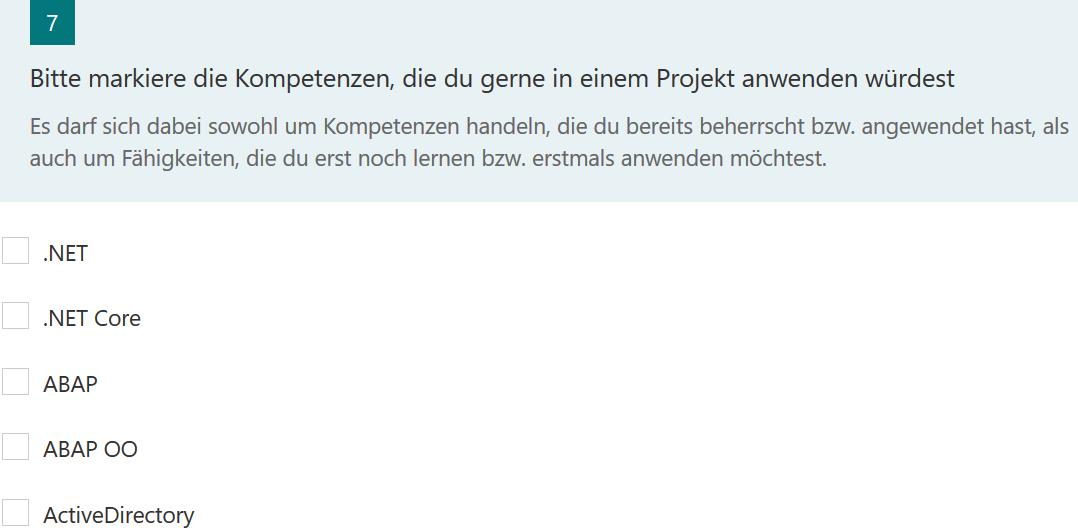
\includegraphics[width=1\textwidth]{gfx/Umfage_Faehigkeiten.png}
	\caption{Auszug aus der Umfrage zur Erhebung der Mitarbeiter-Präferenzen}
	\label{fig:methodik:versuchsaufbau:abb1}
\end{figure}

Die Kompetenzbewertungen der Mitarbeiter und deren Präferenzen dienen im Experiment als Datengrundlage für ein neu entwickeltes, hybrides Empfehlungssystem.

\section{Aufbau des hybriden Empfehlungssystems}
\label{ch:methodik:versuchsaufbau:systemarchitektur}
Das im Rahmen dieser Master-Thesis implementierte Empfehlungssystem basiert auf einer Microservice-Architektur, welche aus drei Diensten und einem Pufferspeicher besteht. Um die Funktionsweisen und Rückgaben der verschiedenen Komponenten des Systems anhand von Beispielen zu erläutern, werden die Mitarbeiter und Kompetenzbewertungen aus Tabelle \ref{tbl:empfehlungssysteme:arbeitsweise:tbl1} verwendet. Dabei wird festgelegt, dass Jane Doe und Max Muster bzw. John Doe und Erika Muster in jeweils einem Team tätig sind. Zusätzlich wird angenommen, dass die Mitarbeiter die Kompetenzen aus Tabelle \ref{tbl:methodik:versuchsaufbau:systemarchitektur:tbl1} präferieren.

\begin{table}[h]
	\centering
	\begin{tabular}{c|c}
		\textbf{Nutzer} & \textbf{Präferierte Fähigkeiten}\\
		\hline
		Jane D.     & HDFS\\
		John D.     & Python, HDFS\\
		Erika M.    & MySQL, Python\\
		Max M.      & HDFS, MySQL
	\end{tabular}
	\caption{Präferierte Fähigkeiten der Beispielnutzer}
	\label{tbl:methodik:versuchsaufbau:systemarchitektur:tbl1}
\end{table}

Sämtliche Komponenten der Microservice-Architektur werden in Form von Docker-Containern ausgeliefert und über Docker Compose orchestriert. Die Dienste kommunizieren untereinander über HTTP. Abbildung \ref{fig:methodik:systemarchitekturn:abb1} zeigt einen Überblick über die Systemarchitektur.

\begin{figure}[h]
	\centering
	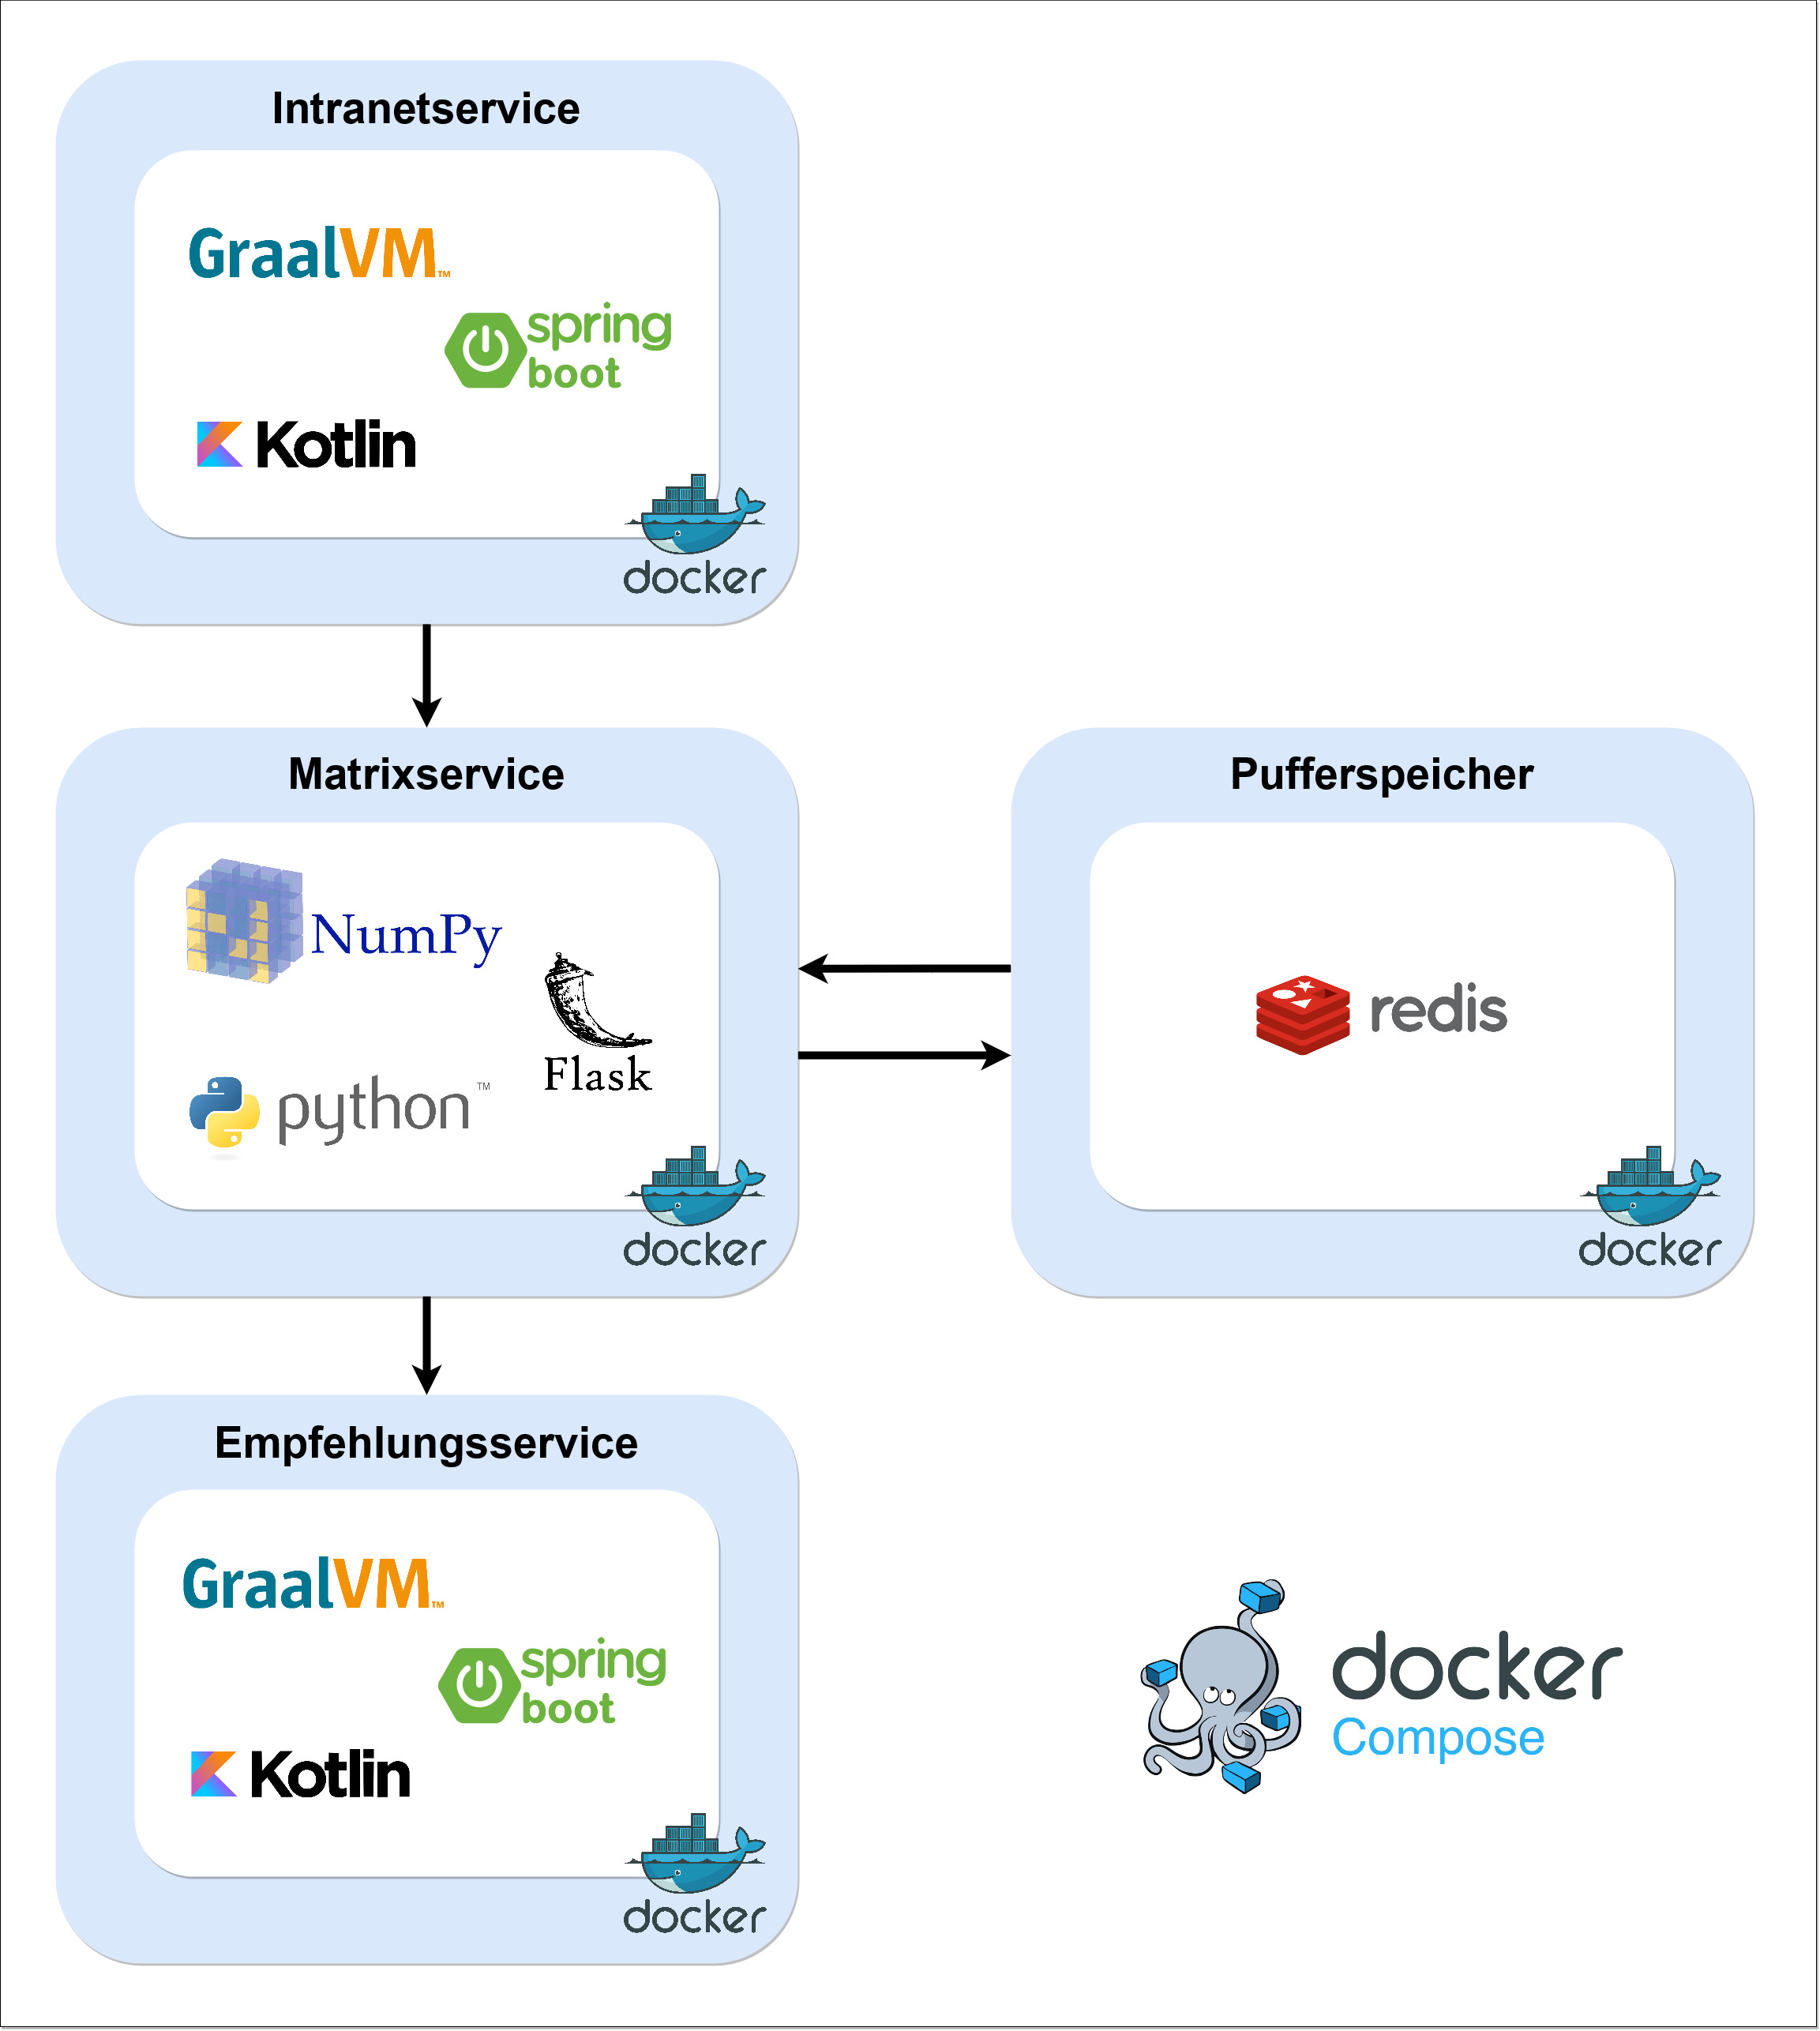
\includegraphics[width=1\textwidth]{gfx/ArchitekturMitLinie.jpg}
	\caption{Systemarchitektur des hybriden Empfehlungssystems}
	\label{fig:methodik:systemarchitekturn:abb1}
\end{figure}

Beim oben in Abbildung \ref{fig:methodik:systemarchitekturn:abb1} dargestellten Intranetservice handelt es sich um einen Dienst, welcher im Rahmen des Experiments das Intranet der EXXETA AG simuliert.

\subsection{Intranetservice}
\label{ch:methodik:versuchsaufbau:systemarchitektur:intranetservice}
Das Intranet der EXXETA AG bietet eine REST-Schnittstelle, welche Informationen über sämtliche Mitarbeiter des Unternehmens in Form von JSON bereitstellt. Über diese können beispielsweise die Kompetenzbewertungen und die Teamzuordnungen der Angestellten ermittelt werden. Einzelne Mitarbeiter sind dabei eindeutig über ihre E-Mail-Adresse identifizierbar.

In der vorliegenden Problemstellung werden nicht die Daten aller Angestellten des Unternehmens benötigt. Der Empfehlungsalgorithmus verwendet ausschließlich die Informationen von denjenigen Mitarbeitern, welche im Rahmen der Umfrage Präferenzen bezüglich eingesetzter Kompetenzen spezifiziert haben.

Die Aufgabe des Intranetservices besteht darin, die Rückgabe der Schnittstelle des Intranets der EXXETA AG mit den erhobenen Präferenzen der Umfrage zu kombinieren. Außerdem werden sämtliche nicht benötigten Informationen und Mitarbeiter zu Gunsten der Datensparsamkeit entfernt. Listing \ref{qc:methodik:versuchsaufbau:daten:qc1} zeigt einen beispielhaften Auszug aus der Rückgabe des Intranetservices.

%\begin{minipage}{\linewidth}
\lstinputlisting[
language=json,
caption=Beispiel für die Rückgabe des Intranetservices (Auszug),
captionpos=b,
label=qc:methodik:versuchsaufbau:daten:qc1
]{gfx/john.json}
%\end{minipage}

Die Implementierung des Intranetservices erfolgte in der Programmiersprache Kotlin. Als Framework wurde Spring Boot in Kombination mit dem GraalVM Native Image-Compiler verwendet, welcher die Startzeit und den benötigten Arbeitsspeicher des Dienstes stark reduziert.

Die Daten des Intranetservices dienen als Eingabe für den Matrixservice, welcher zur Optimierung der Empfehlungsbestimmung die Sparsity- und Kaltstart-Problematik löst.

\subsection{Matrixservice}
\label{ch:methodik:versuchsaufbau:systemarchitektur:matrixservice}
Der Matrixservice basiert auf der Datenstruktur eines Graphen. Hierbei werden die Mitarbeiter der EXXETA AG und deren Fähigkeiten in Form von Knoten dargestellt. Um das Sparsity Problem zu lösen, wird der speicherbasierte Algorithmus von Katz angewendet. Da die Anwendung auch über die Master-Thesis hinaus im Unternehmen zum Einsatz kommen soll, ist insbesondere die Langlebigkeit des Verfahrens vorteilhaft gegenüber modellbasierten Methoden. Sollten sich nach Durchführung des Experiments Daten im Unternehmen verändern oder neue Kompetenzen im Intranet hinzugefügt werden, ist das Empfehlungssystem weiterhin ohne zusätzlichen manuellen Aufwand im Betrieb einsetzbar.

Im Intranet der EXXETA AG ist zu beobachten, dass einige Mitarbeiter keine einzige Fähigkeit beurteilt haben. Hierbei handelt es sich beispielsweise um neue Angestellte oder Mitarbeiter, welche bereits ausgelastet sind und daher vorerst für die Besetzung weiterer Projektpositionen nicht berücksichtigt werden.

Hinsichtlich der Kompetenzbewertungen ist außerdem zu erwarten, dass manche spezialisierte Mitarbeiter ausschließlich Kompetenzen bewerten, über welche kein anderer Angestellter verfügt. Haben Mitarbeiter keine Fähigkeiten bewertet oder verfügen sie ausschließlich über Kompetenzen, welche kein weiterer Angestellter beherrscht, sind diese im Graphen mit keiner anderen Person verbunden. Somit kann ein Kaltstart bei der Empfehlungsbestimmung auftreten.

Um diesem vorzubeugen, werden zusätzlich zu den Fähigkeiten der Mitarbeiter auch deren Teamzuordnungen in Form eines hybriden Ansatzes beachtet. Über dieses Vorgehen sind stets sämtliche Mitarbeiter des Bereichs \JES über den Abteilungsleiter bzw. alle Angestellten der EXXETA AG über den Vorstand miteinander verbunden. Dieses Vorgehen hat zusätzlich den Vorteil, dass die Kompetenzen eines Zielnutzers bei Berechnung des Algorithmus feingranular besser bewertet werden, wenn dessen direkte Kollegen ähnliche Fähigkeiten beherrschen. Dieser Ansatz ist im Falle der EXXETA AG als sinnvoll zu bewerten. Dort sind in der Regel Mitarbeiter mit vergleichbarem fachlichem Hintergrund in einem Team tätig. Auch die Teammanager sind fachliche Führungskräfte, deren Fähigkeiten meist weitgehend repräsentativ für ihre Mitarbeiter sind.

Um eine weitere Erhöhung der algorithmischen Komplexität des Algorithmus von Katz zu vermeiden, werden die Teams nicht als zusätzliche Knoten in den Graphen eingefügt. Die Beziehungen werden stattdessen über direkte Kanten zwischen Kollegen dargestellt. Das Kantengewicht zwischen zwei Teammitgliedern bzw. einem Angestellten zu seinem Manager wird auf \teamgewichtString festgelegt. Dieser Wert wird verwendet, um die Teamzugehörigkeit schwach in die Berechnung mit einzubeziehen, hohe individuelle Kompetenzbewertungen jedoch weiterhin stärker zu gewichten.

Abbildung \ref{fig:methodik:versuchsaufbau:unilateral:abb1} zeigt die Darstellung der Kompetenzen und die Teamzuordnungen der Beispielangestellten in Form eines Graphen.

\begin{figure}[h]
	\centering	
	\begin{tikzpicture}[node distance={32mm}, thick, main/.style = {draw, circle}] 
		\node[main, fill=itemcolor] (MongoDB) {$MongoDB$}; 
		\node[main, fill=itemcolor] (Python) [below right of=MongoDB] {$Python$}; 
		\node[main, fill=itemcolor] (MySQL) [above right of=Python] {$MySQL$}; 
		\node[main, fill=itemcolor] (Java) [below right of=MySQL] {$Java$}; 
		\node[main, fill=itemcolor] (HDFS) [above right of=Java] {$HDFS$}; 
		\node[main, fill=itemcolor] (Spark) [below right of=HDFS] {$Spark$};
		
		\node[main, fill=usercolor] (Jane) [above right of=MongoDB] {$Jane D.$}; 
		\node[main, fill=usercolor] (John) [above left of=HDFS] {$John D.$}; 
		\node[main, fill=usercolor] (Max) [below of=MySQL] {$Max M.$};
		\node[main, fill=usercolor] (Erika) [above right of=HDFS] {$Erika M.$}; 
		
		\draw (Jane) -- node[midway, right] {4} (Python);
		\draw (Jane) -- node[midway, above] {3} (MySQL);
		\draw (Jane) -- node[midway, above] {3} (MongoDB);
		\draw (Jane) -- node[midway, left] {1} (Max);
		
		\draw (John) -- node[midway, right] {1} (HDFS);		
		\draw (John) -- node[midway, right] {3} (Java);
		\draw (John) -- node[midway, above] {2} (MySQL);
		\draw (John) -- node[midway, above] {1} (Erika);
		
		%\path (Erika) edge[bend right=10] node[midway, right] {5} (HDFS); 
		\draw (Erika) -- node[midway, above] {5} (HDFS);
		\draw (Erika) -- node[midway, right] {3} (Spark);
		
		\draw (Max) -- node[midway, above] {2} (Java);
		\draw (Max) -- node[midway, above] {3} (Python);
		\draw (Max) -- node[midway, right] {1} (MySQL);
	\end{tikzpicture}
	
	\caption{Graph aus Abbildung \ref{fig:empfehlungssysteme:cf:speicherbasiert:abb2} mit zusätzlicher Teamzuordnung}
	\label{fig:methodik:versuchsaufbau:unilateral:abb1}
\end{figure}

%Im Graphen aus Abbildung \ref{fig:methodik:versuchsaufbau:unilateral:abb1} ist zu erkennen, dass die ganzzahligen Bewertungen der Kompetenzen des Intranets um eins erhöht wurden. Somit reichen die Beurteilungen beherrschter Fähigkeiten anstelle von \nullWert bis fünf nun von eins bis sechs. Auf diese Weise verfügen ausschließlich nicht beherrschte Kompetenzen über eine Bewertung von \nullWert und stellen somit keine Kante im Graphen da.
Die Daten des Graphen aus Abbildung \ref{fig:methodik:versuchsaufbau:unilateral:abb1} dienen als Grundlage zur Berechnung des Katz-Algorithmus anhand von Gleichung \ref{frml:methodik:versuchsaufbau:systemarchitektur:matrixservice:formel1}, welche in Kapitel \ref{ch:empfehlungssysteme:cf:speicherbasiert} vorgestellt wurde:
\begin{equation}
	(I - \beta * M)^{-1} - I
	\label{frml:methodik:versuchsaufbau:systemarchitektur:matrixservice:formel1}
\end{equation}
Im Matrixservice wird der Wert von $\beta$ über folgende Gleichung \ref{frml:methodik:versuchsaufbau:grundlegend:formel1} bestimmt:
\begin{equation}
	\beta = \frac{1/\lambda}{\nenner}
	\label{frml:methodik:versuchsaufbau:grundlegend:formel1}
\end{equation}
Durch das in Gleichung \ref{frml:methodik:versuchsaufbau:grundlegend:formel1} dargestellte Vorgehen ist sichergestellt, dass $\beta$ auch bei sich ändernder Datenlage stets kleiner als $1/\lambda$ ist. Wie in Kapitel \ref{ch:empfehlungssysteme:cf:speicherbasiert} erläutert, entspricht $\lambda$ dem größten Eigenwert der Adjazenzmatrix $M$ des Graphen. Aufgrund der Division durch \nenner ist $\beta$ stets so groß, dass von einem Zielnutzer weit entfernte Knoten noch in die Berechnung einbezogen werden, nahe Fähigkeiten jedoch stärker gewichtet werden. Auf diese Weise erhalten die Knoten ein höheres Gewicht, welche direkt mit dem Zielnutzer in Verbindung stehen.

Wie in Kapitel \ref{ch:empfehlungssysteme:cf:speicherbasiert} beschrieben, ändern sich bei Berechnung des Verfahrens von Katz die Fähigkeitsbewertungen. Allerdings befinden sich die Beurteilungen, welche ursprünglich einem gemeinsamen Kompetenzniveau entsprachen, auch nach Berechnung des Algorithmus auf einem vergleichbaren Niveau. Die Werte innerhalb eines Kompetenzbereichs sind lediglich feingranular unterschiedlich. Dieses Phänomen ist in Tabelle \ref{tbl:methodik:versuchsaufbau:unilateral:tbl1} zu beobachten. Dort sind die Bewertungen der Fähigkeit MySQL aus Abbildung \ref{fig:methodik:versuchsaufbau:unilateral:abb1} vor und nach der Berechnung des Katz-Algorithmus eingetragen. Gleiche Kompetenzniveaus sind in Tabelle \ref{tbl:methodik:versuchsaufbau:unilateral:tbl1} durch einheitliche Hintergrundfarben gekennzeichnet.

\begin{table}[h]
	\centering
	\begin{tabular}{c|c|c|c}
		\textbf{Name} & \textbf{Kompetenzniveau} & \textbf{Original-Bewertung} & \textbf{Matrix-Ergebnis} \\
		\hline
		\rowcolor{exxetagray}Erika M. & Keine Kenntnisse & 0 & 0.42\\
		\hline
		\rowcolor{itemcolor}Max M.    & Grundkenntnisse  & 1 & 1.32\\
		\rowcolor{itemcolor}John D.   & Grundkenntnisse  & 2 & 0.92\\
		\rowcolor{itemcolor}Jane D.   & Grundkenntnisse  & 3 & 2.10
	\end{tabular}
	\caption{Ergebnisse des Katz-Algorithmus für die Kompetenz MySQL im Graphen aus Abbildung \ref{fig:methodik:versuchsaufbau:unilateral:abb1}}
	\label{tbl:methodik:versuchsaufbau:unilateral:tbl1}
\end{table}

Wie in Tabelle \ref{tbl:methodik:versuchsaufbau:unilateral:tbl1} zu erkennen, haben Max Muster, Jane und John Doe auch nach Berechnung des Katz-Algorithmus vergleichbare Bewertungen. Es kann interpretiert werden, dass sich die drei Beispielangestellten ähnlich gut mit MySQL auskennen, Jane Doe die Fähigkeit jedoch wenig besser beherrscht als ihre beiden Kollegen. Die Ergebnisse der letzten Spalte von Tabelle \ref{tbl:methodik:versuchsaufbau:unilateral:tbl1} werden als unilateraler Empfehlungswert betrachtet. Dieser wird zu einem späteren Zeitpunkt im Empfehlungsservice benötigt.

Präferiert einer der Mitarbeiter in Tabelle \ref{tbl:methodik:versuchsaufbau:unilateral:tbl1} eine Fähigkeit, ist davon auszugehen, dass dessen Bewertung aufgrund seiner Motivation höher ist, als bei den anderen Angestellten innerhalb seines Kompetenzniveaus. Aus diesem Grund bestimmt der Matrixservice in einem weiteren Rechenschritt für jede Fähigkeit die höchste Bewertung innerhalb jedes der drei Kompetenzniveaus aus Tabelle \ref{tbl:methodik:versuchsaufbau:systemarchitektur:matrixservice:tbl1}. Favorisiert ein Mitarbeiter eine bestimmte Fähigkeit, addiert der Dienst die höchste Bewertung des Kompetenzniveaus des Mitarbeiters zu dessen Beurteilung. Durch dieses Vorgehen verbleiben die Angestellten bei ihrer ursprünglichen Bewertung, wenn sie die betrachtete Kompetenz nicht präferieren. Wünschen sich mehrere Mitarbeiter dagegen die Fähigkeit im Projekt anzuwenden, erhalten sie innerhalb des Kompetenzniveaus eine höhere Positionierung. Hierbei bleibt die ursprüngliche Reihenfolge der Angestellten gleich, sodass Projektmanager als ersten Vorschlag den fähigsten und zugleich motiviertesten Angestellten erhalten. Somit werden gemäß des ergänzenden \acp{PEFit} gleichzeitig die Präferenzen von Projektmanagern und Mitarbeitern betrachtet. Die Ergebnisse des beschriebenen Rechenschritts werden als bilateraler Empfehlungswert gespeichert. Die unilateralen und bilateralen Empfehlungswerte für die Beispielmitarbeiter sind in Tabelle \ref{tbl:methodik:versuchsaufbau:unilateral:tbl3} dargestellt.

\begin{table}[h]
	\centering
	\begin{tabular}{c|c|c|c|c|c}
		\textbf{Name} & \textbf{Niveau} & \textbf{Orig.-Bew.} & \textbf{Unil.-Empf.} & \textbf{Präferenz} & \textbf{Bil.-Empf.}\\
		\hline
		\rowcolor{exxetagray}Erika M. & Keine K. & 0 & 0.42 & Ja   & 0.84\\
		\hline
		\rowcolor{itemcolor}Max M.    & Grundk.  & 1 & 1.32 & Ja   & 3.42\\
		\rowcolor{itemcolor}John D.   & Grundk.  & 2 & 0.92 & Nein & 0.92\\
		\rowcolor{itemcolor}Jane D.   & Grundk.  & 3 & 2.10 & Nein & 2.10
	\end{tabular}
	\caption{Ergebnisse des Katz-Algorithmus für die Kompetenz MySQL im Graphen aus Abbildung \ref{fig:methodik:versuchsaufbau:unilateral:abb1}}
	\label{tbl:methodik:versuchsaufbau:unilateral:tbl3}
\end{table}

In Tabelle \ref{tbl:methodik:versuchsaufbau:unilateral:tbl3} ist zu erkennen, dass sich die bilateralen Empfehlungswerte von Erika bzw. Max Muster von den unilateralen Ergebnissen unterscheiden. Ursächlich ist, dass beide Mitarbeiter die Fähigkeit MySQL präferieren. Da Erika Muster in der Tabelle als geeignetste Mitarbeiterin auf ihrem Kompetenzniveau für die Fähigkeit MySQL betrachtet wird, verdoppelt sich ihre Beurteilung bei der Bestimmung des bilateralen Empfehlungswertes. Jane Doe ist dagegen die potentiell fähigste Angestellte mit Grundkenntnissen in MySQL. Da Max Muster diese Kompetenz präferiert, wird bei Berechnung des bilateralen Empfehlungswertes sein Ergebnis des Katz-Algorithmus zu Jane Does Resultat addiert. Durch diesen Rechenschritt befinden sich sämtliche Bewertungen der Fähigkeit MySQL auch nach Bestimmung des bilateralen Empfehlungswertes auf einem vergleichbaren Niveau. Lediglich die Reihenfolge der Mitarbeiter wurde innerhalb der Kompetenzstufen verändert.%Beispielsweise wurde die Beurteilung von Erika Muster erhöht. Dennoch ist diese geringer als die Bewertung von John Doe, welcher über die geringste Beurteilung des nächst höheren Kompetenzbereichs verfügt.

Der Matrixservice gibt die uni- und bilateralen Empfehlungswerte in Form von JSON zurück. Listing \ref{qc:methodik:versuchsaufbau:daten:qc2} zeigt beispielhaft eine Ausgabe des Matrixservice, welche einen Auszug der Daten von John Doe enthält.

%\begin{minipage}{\linewidth}
\lstinputlisting[
language=json,
caption=Beispiel für die Rückgabe des Matrixservices (Auszug),
captionpos=b,
label=qc:methodik:versuchsaufbau:daten:qc2
]{gfx/john-matrix.json}
%\end{minipage}

In Listing \ref{qc:methodik:versuchsaufbau:daten:qc2} ist zu erkennen, dass jede Fähigkeit vier Attribute besitzt. Die Werte von uni- bzw. bilateralLevel stehen für die uni- bzw. bilateralen Empfehlungswerte. Das Attribut preference zeigt an, ob der Mitarbeiter die Kompetenz präferiert. Der Wert von originalLevel gibt die originale Kompetenzbewertung des Angestellten aus dem Intranet wieder, welche den Kantengewichten im Graphen entsprechen.

Da die Berechnung des Katz-Algorithmus eine hohe algorithmische Komplexität aufweist, speichert der Matrixservice die Ergebnisse seiner Berechnung zur effizienteren Vorschlagsbestimmung in einem Pufferspeicher zwischen. Somit muss der Dienst die Berechnung erst bei veränderter Datenlage im Unternehmen erneut ausführen. Dieses Vorgehen kombiniert die Vorteile von speicher- und modellbasierten Empfehlungsansätzen: Wie bei speicherbasierten Verfahren üblich, greift der Matrixservice stets auf die aktuellen Daten des Unternehmens zurück. Durch die Zwischenspeicherung der Ergebnisse wird gleichzeitig eine bei modellbasierten Verfahren zu erwartende Effizienz bei der Empfehlungsgenerierung erzielt.

Die Implementierung des Matrixservices erfolgte in der Programmiersprache Python. Eingesetzt wurden dabei das Framework Flask und das Paket Numpy, welches die Matrixberechnungen unterstützt. Als Pufferspeicher kommt der Schlüssel-Wert-Speicher Redis zum Einsatz.

Die finale Empfehlungsbestimmung anhand der Ausgabe des Matrixservices erfolgt abschließend im Empfehlungsservice.

\subsection{Empfehlungsservice}
\label{ch:methodik:versuchsaufbau:systemarchitektur:empfehlungsservice}
Der Empfehlungsservice enthält eine Schnittstelle, über welche Projektmanager die für offene Projektpositionen benötigten Fähigkeiten eingeben können. Wie in Listing \ref{qc:methodik:versuchsaufbau:systemarchitektur:empfehlungsservice:qc1} dargestellt, müssen diese hierbei den Namen jeder Kompetenz angeben und das gesuchte Fähigkeitsniveau über das boolsche Attribut expert spezifizieren. 

%\begin{minipage}{\linewidth}
\lstinputlisting[
language=json,
caption=Beispiel für eine Eingabe in den Empfehlungsservice,
captionpos=b,
label=qc:methodik:versuchsaufbau:systemarchitektur:empfehlungsservice:qc1
]{gfx/project-input.json}
%\end{minipage}

Bei der unilateralen Vorschlagsgenerierung bestimmt der Empfehlungsservice gemäß des Anforderungen-Fähigkeiten Fits ausschließlich Angestellte, welche die höchste Eignung für die Ansprüche des Projektmanagers aufweisen. Hierbei wird angenommen, dass die Verantwortlichen anstreben, offene Projektpositionen mit fachlich optimal passenden Mitarbeitern zu besetzen. Folglich vermeiden sie sowohl eine Über- als auch eine Unterqualifizierung ihrer Angestellten. Aus diesem Grund wird der \ac{PEFit} anhand von Kurve B in Abbildung \ref{fig:methodik:versuchsaufbau:unilateral:abb2} bestimmt. Dabei wird die quadrierte Differenzberechnung angewendet.

\begin{figure}[h]
	\centering
	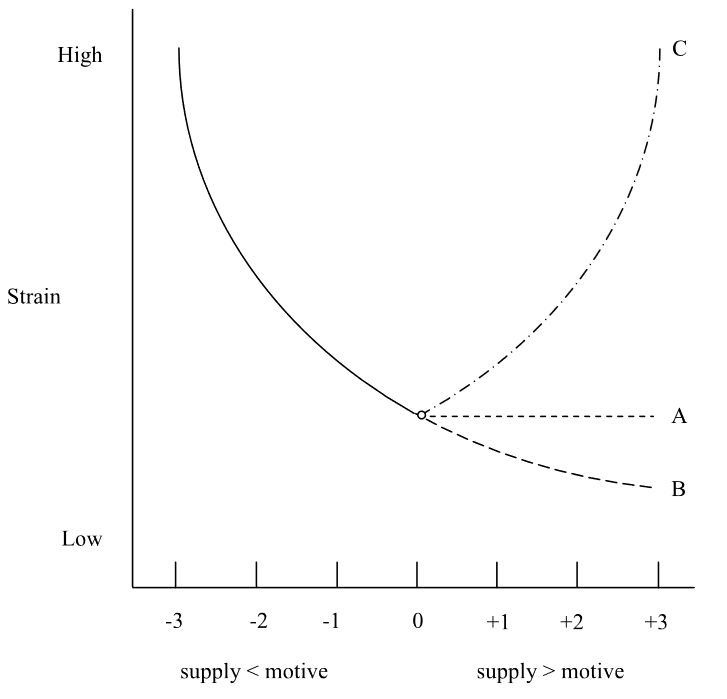
\includegraphics[width=0.75\textwidth]{gfx/ueberschuss_supply_motive.png}
	\caption{Auswirkungen eines Bedürfnisse-Angebote Misfits\\(Eigene Darstellung in Anlehnung an \cite[S. 23]{edwards:2008})}
	\label{fig:methodik:versuchsaufbau:unilateral:abb2}
\end{figure}

Wird anhand der Daten aus Tabelle \ref{tbl:methodik:versuchsaufbau:unilateral:tbl3} ein Mitarbeiter mit Grundkenntnissen in MySQL gesucht, wird der Angestellte mit dem höchsten Wert im gesuchten Kompetenzbereich als geeignetster Kandidat betrachtet. Im vorliegenden Beispiel wäre somit Jane Doe die qualifizierteste Mitarbeiterin für die Suche nach einem Angestellten mit Grundkenntnissen im Umgang mit MySQL. Ihre Bewertung dient daher bei der Bestimmung des \acp{PEFit} als Nullpunkt in Abbildung \ref{fig:methodik:versuchsaufbau:unilateral:abb2}.

Ist kein Mitarbeiter im gesuchten Kompetenzbereich vorhanden, führt der Empfehlungsservice eine Ausnahmebehandlung durch. Wird hierbei nach Grundkenntnissen in einer bestimmten Fähigkeit gesucht und kein passender Kandidat gefunden, wird der wenig qualifizierteste Angestellte auf fortgeschrittenem Niveau als Referenz genutzt. Wird erfolglos nach Mitarbeitern mit fortgeschrittenen Kenntnissen gesucht, wird der am Besten qualifizierte Kandidat mit Grundkenntnissen als Referenz verwendet. Sind ausschließlich Mitarbeiter ohne Kenntnisse vorhanden, wird die gesuchte Kompetenz übersprungen, da in diesem Fall kein Mitarbeiter im Graphen mit dieser Fähigkeit verbunden sein kann und somit alle Kantengewichte \nullWert sein müssen.

Tabelle \ref{tbl:methodik:versuchsaufbau:unilateral:tbl2} zeigt das Ergebnis der unilateralen Empfehlungsbestimmung für die Beispielmitarbeiter und das Projekt aus Listing \ref{qc:methodik:versuchsaufbau:systemarchitektur:empfehlungsservice:qc1}. Die vollständige Berechnung kann in Anhang \ref{ch:nebenrechnungen:unilateral} nachvollzogen werden.

\begin{table}[h]
	\centering
	\begin{tabular}{c|c|c}
		\textbf{Positionierung} & \textbf{Mitarbeiter} & \textbf{Abweichung}\\
		\hline
		1 & Jane D.  & 0.1\\
		2 & Max M.   & 1.6\\
		3 & John D.  & 5.9\\
		4 & Erika M. & 10.4
	\end{tabular}
	\caption{Ergebnisliste der unilateralen Empfehlungsbestimmung für ein Beispielprojekt}
	\label{tbl:methodik:versuchsaufbau:unilateral:tbl2}
\end{table}

Die letzte Spalte in Tabelle \ref{tbl:methodik:versuchsaufbau:unilateral:tbl2} gibt die aufsummierten quadrierten Abweichungen der einzelnen Fähigkeitsbewertungen der Mitarbeiter von den optimalen Kompetenzbeurteilungen an. Je kleiner die Abweichung ist, desto geeigneter sind die Mitarbeiter folglich für die zu besetzende Projektposition. In den Ergebnissen ist zu erkennen, dass für das gesuchte Projekt aus Listing \ref{qc:methodik:versuchsaufbau:systemarchitektur:empfehlungsservice:qc1} Jane Doe als geeignetste Mitarbeiterin empfohlen wird.

Ähnlich zu den unilateralen Ergebnissen bestimmt der Empfehlungsservice auch die bilateralen Resultate. Dabei bezieht der Dienst neben dem Anforderungen-Fähigkeiten Fit auch die Präferenzen der Mitarbeiter bzw. die Bedürfnisse-Angebote Kongruenz zur Bestimmung eines vollständigen \acp{PEFit} in die Berechnung mit ein. Hierbei werden aus der Rückgabe des Matrixservice aus Listing \ref{qc:methodik:versuchsaufbau:daten:qc2} anstelle der unilateralen die bilaterale Empfehlungswerte verwendet. Durch dieses Vorgehen werden, wie von \textcite[S. 51ff.]{edwards:1991} in Kapitel \ref{ch:personEnvironmentFit:regressionsgleichungen} gefordert, die Präferenzen von Projektmanagern und Angestellten getrennt voneinander in die Berechnung einbezogen.

Hinsichtlich der Linien aus Abbildung \ref{fig:methodik:versuchsaufbau:unilateral:abb2} wird auch von den Mitarbeitern erwartet, dass diese Über- und Unterforderung im Projekt vermeiden möchten. Daher wird auch bei dieser Berechnung Kurve B über die quadrierte Differenzberechnung implementiert.

Tabelle \ref{tbl:methodik:versuchsaufbau:bilateral:tbl2} zeigt die Ergebnisse der bilateralen Empfehlungsbestimmung für das Projekt aus Listing \ref{qc:methodik:versuchsaufbau:systemarchitektur:empfehlungsservice:qc1}. Die vollständige Berechnung kann in Anhang \ref{ch:nebenrechnungen:bilateral} nachvollzogen werden.

\begin{table}[h]
	\centering
	\begin{tabular}{c|c|c}
		\textbf{Positionierung} & \textbf{Mitarbeiter} & \textbf{Abweichung}\\
		\hline
		1 & Max M.   & 1.4\\
		2 & Jane D.  & 2.1\\
		3 & John D.  & 8.0\\
		4 & Erika M. & 9.8
	\end{tabular}
	\caption{Ergebnisliste der bilateralen Empfehlungsbestimmung für ein Beispielprojekt}
	\label{tbl:methodik:versuchsaufbau:bilateral:tbl2}
\end{table}

In Tabelle \ref{tbl:methodik:versuchsaufbau:bilateral:tbl2} ist zu erkennen, dass Max Muster aufgrund seiner Präferenzen besser positioniert sind, als zuvor in Tabelle \ref{tbl:methodik:versuchsaufbau:unilateral:tbl2}. Außerdem hat sich der Abstand von Erika Muster auf John Doe verringert. Außerdem ist zu erkennen, dass der Empfehlungsservice die Angestellten stets nach geringster Abweichung sortiert.

Wie der Intranetservice wurde auch der Empfehlungsservice in der Programmiersprache Kotlin implementiert. Ebenfalls kamen das Framework Spring Boot und der GraalVM Native Image-Compiler zum Einsatz. Ein Auszug aus der vollständigen Ausgabe des Empfehlungsservices für die Projektanfrage aus Listing \ref{qc:methodik:versuchsaufbau:systemarchitektur:empfehlungsservice:qc1} ist in Listing \ref{qc:methodik:versuchsaufbau:daten:qc3} dargestellt.

%\begin{minipage}{\linewidth}
\lstinputlisting[
language=json,
caption=Beispiel für die Rückgabe des Empfehlungsservices (Auszug),
captionpos=b,
label=qc:methodik:versuchsaufbau:daten:qc3
]{gfx/john-empfehlungsservice.json}
%\end{minipage}

In Listing \ref{qc:methodik:versuchsaufbau:daten:qc3} ist zu erkennen, dass zu jedem Mitarbeiter die berechnete Abweichung unter der Bezeichnung recommendationValue zurückgegeben wird. Außerdem kann für jeden Angestellten entnommen werden, ob diese die jeweiligen gesuchten Fähigkeiten präferieren und welche Bewertung diese im Intranet für die Kompetenzen abgegeben haben.

Die Ausgaben des Empfehlungsservices dienen im Rahmen der vorliegenden Master-Thesis als Grundlage für eine Fallstudie, welche zur Beantwortung der Forschungsfrage mit Projektmanagern und Mitarbeitern des Fachbereichs \JES der EXXETA AG durchgeführt wird.

\section{Geplante Fallstudie}
\label{ch:methodik:evaluation}
Vor Durchführung der Fallstudie definiert ein Projektmanager des Fachbereichs \JES fünf Projektpositionen. Dieser betrachtet die Stellen als repräsentativ für häufige Kundenanfrage an die Abteilung. Abbildung \ref{fig:methodik:evaluation:abb2} zeigt die vordefinierten Projektpositionen.

\begin{figure}[h]
	\centering
	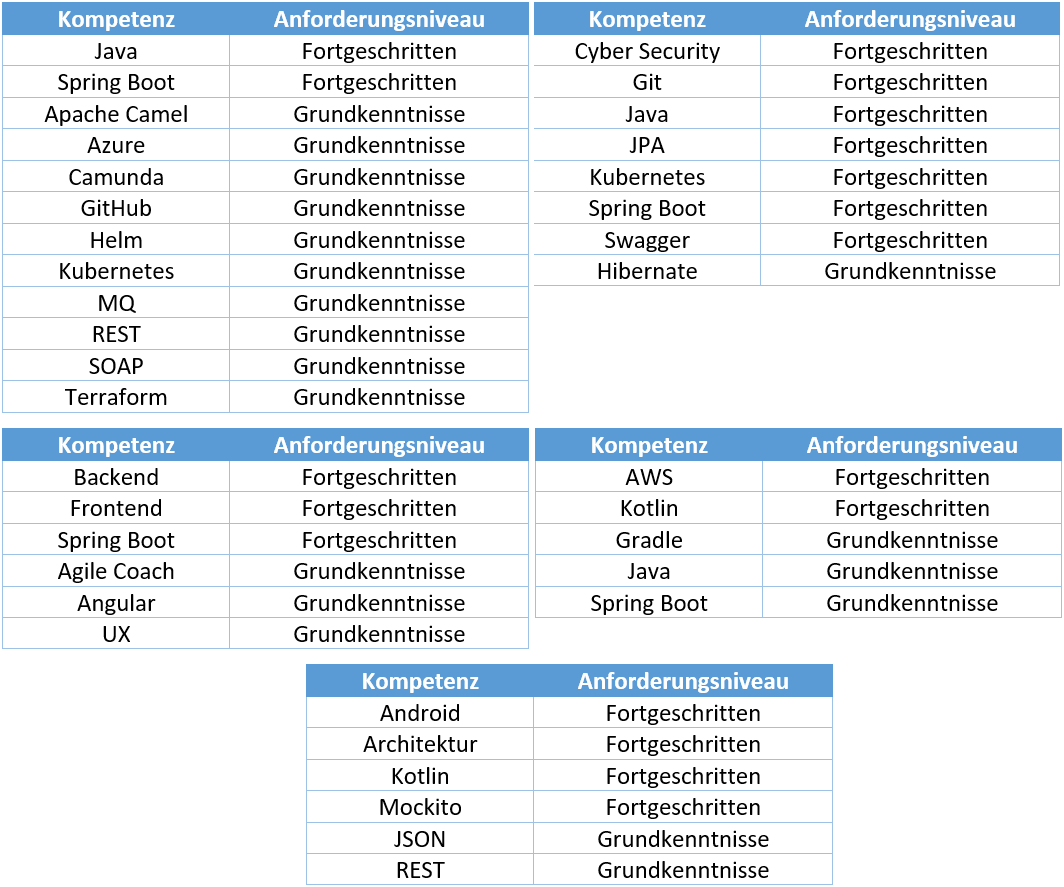
\includegraphics[width=1.0\textwidth]{gfx/Projekt.png}
	\caption{Für die Evaluation definierte Projektpositionen}
	\label{fig:methodik:evaluation:abb2}
\end{figure}

Die in Abbildung \ref{fig:methodik:evaluation:abb2} dargestellten Projektpositionen dienen als Grundlage für eine Befragung der Mitarbeiter und der Projektmanager des Bereichs \JES.

\section{Befragung der Projektmitarbeiter}
\label{ch:methodik:evaluation:mitarbeiter}
Wie anhand von Abbildung \ref{fig:methodik:versuchsaufbau:abb1} beschrieben, werden die Mitarbeiter der EXXETA AG in der Umfrage gebeten, ihre präferierten Kompetenzen auszuwählen. In dieser Befragung erhalten diese zusätzlich die vordefinierten Projektpositionen aus Abbildung \ref{fig:methodik:evaluation:abb2}. Hierbei werden diese aufgefordert, ihre Zufriedenheit mit einer Tätigkeit auf den dargestellten Projektpositionen auf einer vierstufigen Skala zu bewerten. Diese wird gewählt, um neutrale Beurteilungen zu vermeiden. Abbildung \ref{fig:methodik:evaluation:abb1} zeigt einen Auszug aus der Umfrage, welchem die Aufgabenstellung zu entnehmen ist.

\begin{figure}[h]
	\centering
	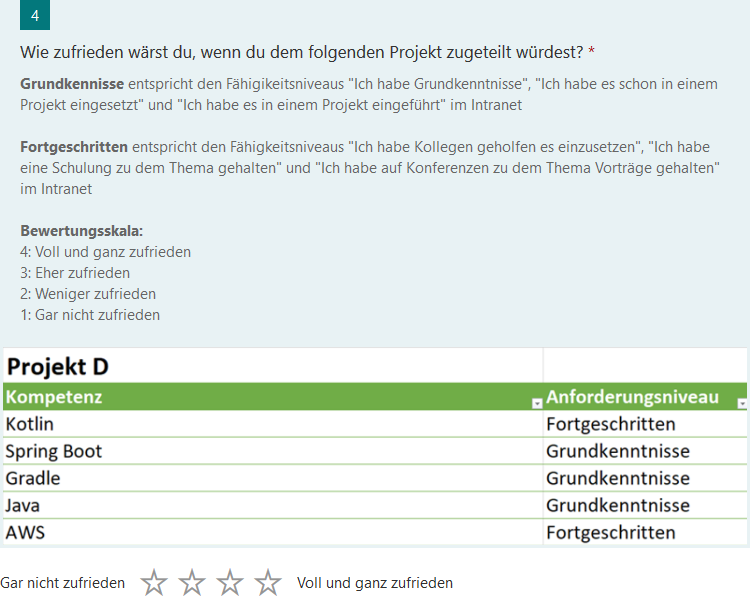
\includegraphics[width=1\textwidth]{gfx/projekt-umfrage.png}
	\caption{Bewertung eines Projektes im Fragebogen der Mitarbeiter}
	\label{fig:methodik:evaluation:abb1}
\end{figure}

Nach Abschluss der Umfrage wird überprüft, ob das bilaterale Empfehlungssystem die Angestellten für die Projektpositionen höher positioniert, bei welchen diese eine hohe Zufriedenheit erwarten bzw. niedriger positioniert, wenn diese eine geringe Zufriedenheit prognostizieren.

Zusätzlich wird überprüft, wie die Angestellten einer möglichen Unterforderung bei der Projekttätigkeit gegenüber stehen. Die entsprechende Frage ist in Abbildung \ref{fig:methodik:evaluation:abb3} dargestellt.

\begin{figure}[h]
	\centering
	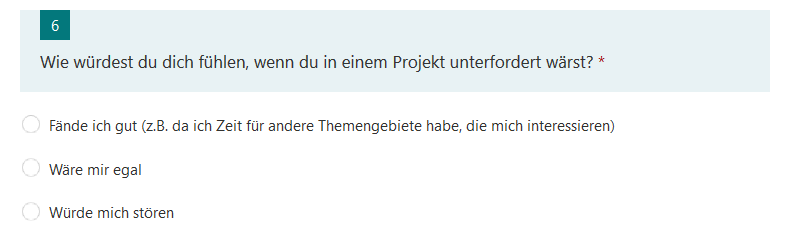
\includegraphics[width=1\textwidth]{gfx/umfrage-mitarbeiter-unterforderung.png}
	\caption{Frage zur Unterforderung der Mitarbeiter im Fragebogen der Angestellten}
	\label{fig:methodik:evaluation:abb3}
\end{figure}

Die Frage aus Abbildung \ref{fig:methodik:evaluation:abb3} dient der Überprüfung der Hypothese, dass Mitarbeiter sowohl eine Unter- als auch eine Überforderung bei der Projekttätigkeit vermeiden möchten. Diese Annahme diente als Grundlage, Kurve B aus Abbildung \ref{fig:methodik:versuchsaufbau:unilateral:abb2} bei Bestimmung des \acp{PEFit} in Form der quadrierten Differenzberechnung zu implementieren.

\section{Befragung der Projektmanager}
\label{ch:methodik:evaluation:manager}
Neben der Befragung der Angestellten wird auch eine Umfrage unter Projektmanagern durchgeführt. Diese erhalten die fünf qualifiziertesten Mitarbeiter jedes Empfehlungsansatzes für die vorausgewählten Projektpositionen in Form von Listen. Anschließend bewerten sie auf einer vordefinierten Skala, von welchen Angestellten sie eine höhere Arbeitsleistung für die jeweiligen Stellen erwarten. Abbildung \ref{fig:methodik:evaluation:manager:abb1} zeigt einen Auszug aus der Befragung.

\begin{figure}[h]
	\centering
	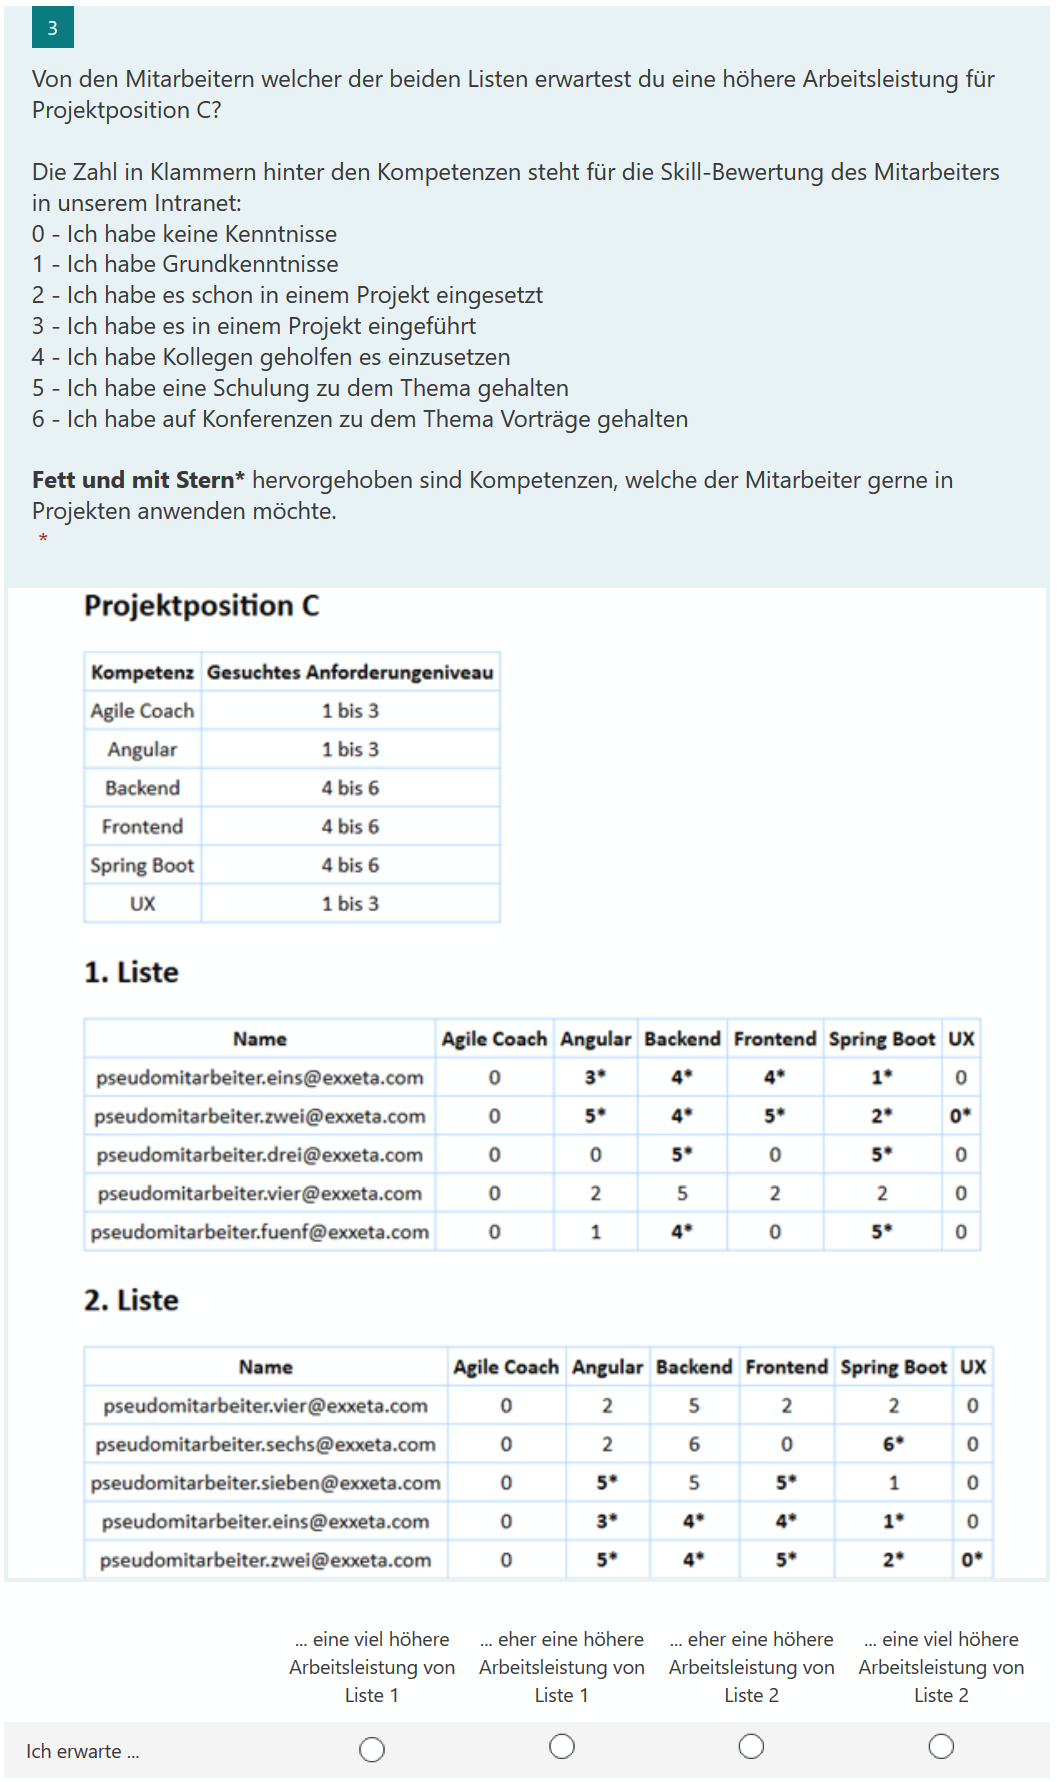
\includegraphics[width=0.75\textwidth]{gfx/projekt-c-liste-pseudonym.png}
	\caption{Frage zur Bewertung der unterschiedlichen Listen\\
	(Klarnamen wurden aus Datenschutzgründen pseudonymisiert)}
	\label{fig:methodik:evaluation:manager:abb1}
\end{figure}

Wie in Abbildung \ref{fig:methodik:evaluation:manager:abb1} dargestellt, können die Projektmanager nicht erkennen, welche Liste durch den unilateralen bzw. den bilateralen Empfehlungsansatz erzeugt wurde.

Im Anschluss an die Umfrage wird evaluiert, wie die Projektmanager die erwartete Leistung der vorgeschlagenen Angestellten des bilateralen Ansatzes im Vergleich zur unilateralen Variante bewerten.

Zusätzlich wird auch in der Umfrage unter den Projektmanagern validiert, ob diese eine Unterforderung ihrer Angestellten bei der Besetzung offener Projektpositionen vermeiden möchten. Die entsprechende Frage ist in Abbildung \ref{fig:methodik:evaluation:manager:abb3} dargestellt.

\begin{figure}[h]
	\centering
	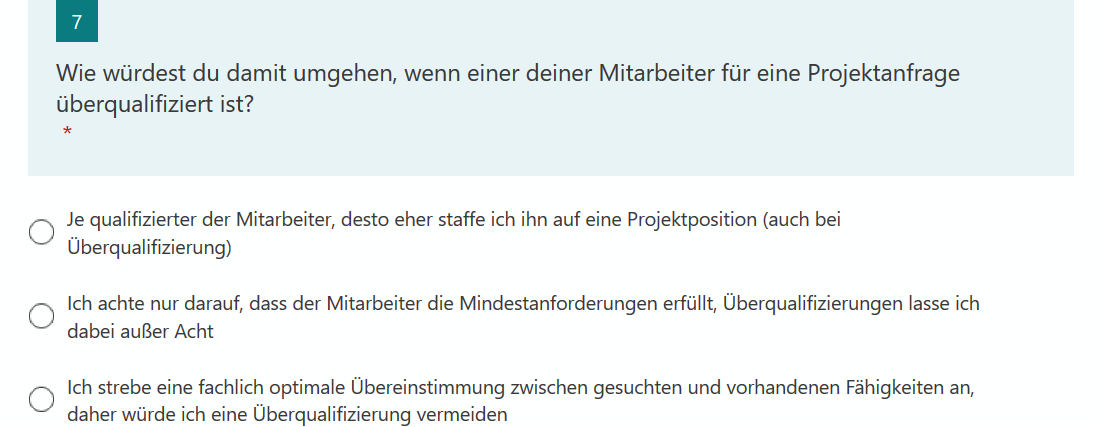
\includegraphics[width=1\textwidth]{gfx/umfrage-projektmanager-unterforderung.png}
	\caption{Frage zur Unterforderung der Mitarbeiter im Fragebogen der Projektmanager}
	\label{fig:methodik:evaluation:manager:abb3}
\end{figure}
\shorthandon{"}